\chapter{Introduction}
\label{ch:intro}

We live in a world where technologies have become vital for our welfare and success.
The internet, for instance, gave us the ability of efficiently exchange information on a global scale.
However, in contrast to its original design, the internet and in particular the world wide web is becoming increasingly centralised.
The domain name system (root name server), certificate authorities (root CA), to name a few, carry enormous responsibilities and are a central point of failure.
The  same can be said for many other services such are online marketplaces,
cloud services, hospitality services and even our banking system.
The 2008 financial crisis is an example of the banking system making poor choices which resulted in a
decline in consumer wealth in the order of trillions~\cite{financialcrisis} and led to the European debt crisis.

Ironically, also in 2008, Satoshi Nakamoto published the Bitcoin whitepaper~\cite{bitcoin}.
Which, for the first time, gave us a simple banking system in the form of a distributed ledger, also known as blockchain.
It needs no central control but still incorruptable with high probability even if there are malicious parties that aim to undermine the system.

The primary innovations are (1) its consensus model which prevents double spending,
and (2) its incentive mechanism that encourages anyone (with adaquate hardware) to participate in the network and keep it running.
The double spending problem can be seen as an inconsistency issue.
For example, $C$ has 5 units of currency in her account.
If $C$ can simultaneously claim that she transferred 5 units to $A$ but also 5 units to $B$, then the system is inconsistent.
Bitcoin and many of its derivatives (e.g. Litecoin\footnote{\url{https://litecoin.org}} and Dogecoin\footnote{\url{http://dogecoin.org}}) solve the inconsistency problem with a consensus algorithm.
The goal of the algorithm is to reach agreement on a set of valid transactions. 
This effectively eliminates inconsistencies.

In Bitcoin's case, the consensus algorithm is called \emph{proof-of-work}.
Where miners (parties that runs the Bitcoin network) collect transactions and compete in solving a puzzle.
The puzzle is easy to verify but difficult to solve.
Only the miner that solves it can generate a valid block containing all the collected transactions.
The miner is also rewarded with new coins and transaction fees.
It is important to note that every block, that is the solution of the puzzle,
depends on the previous block.
Hence the name blockchain.
This property ensures malicious nodes cannot easily rewrite history if they do not have a majority of the network's computing power.
Consequently, it is unlikely for more than one blockchain to exist in the network for a long period of time.
Thus every party sees a consistent blockchain which solves the double spending problem.
% Further, due to the reward mechanism,
% people are incentivised to act as miners and keep the system running.

Bitcoin has had its ups and downs, but over it has grown into an enormous system.
Its power consumption is as high as Republic of Ireland~\cite{o2014bitcoin}.
Its market capitalisation, at the time of writing, is over 60 billion USD~\cite{bitcoinmarketcap} and growing (\Cref{fig:market-cap}).
\begin{figure}[h]
\centering
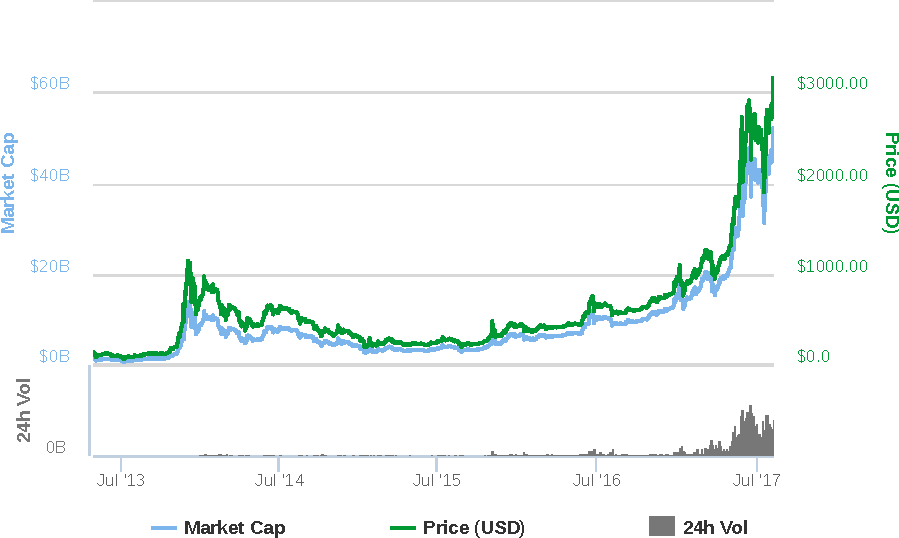
\includegraphics[width=\textwidth]{market-cap}
\caption{Market capitalisation and price of Bitcoin, graph is extracted from~\cite{bitcoinmarketcap}.}
\label{fig:market-cap}
\end{figure}
Many online marketplaces are using Bitcoin, for example Steam\footnote{\url{https://store.steampowered.com/}} and even Amazon\footnote{Not directly, but via \url{https://purse.io/}.}.
Due to its success, people from many different disciplines began investigating in way to use blockchain technology.
This includes finance~\cite{finance}, heathcare~\cite{healthcare}, logistics~\cite{supplychain} and energy~\cite{energy}.

Sadly, as traditional blockchain systems began to gain popularity,
their limitations also became apparent.
Bitcoin has the infamous 7 transactions per second upper bound~\cite{vukolic2015quest}.
This is due to the fact that blocks are fixed to 1 MB are only generated on average every 10 minutes.
Since every Bitcoin transaction is at least 250 bytes, it computes to about 7 transactions per second.
Due to this limitation, it is not uncommon to see a long backlog of about 20,000 transactions\footnote{\url{https://blockchain.info/unconfirmed-transactions/}}.
A few months ago the backlog even reached 100,000, which meant new transactions would take at least 11 hours to be written to the blockchain~\cite{bitcoinbacklog}.
This issue has plagued the Bitcoin community for some time and is the root cause for the block size debate, which some calls it a civil war~\cite{bitcoincivilwar}.
Parties that are for the increase in block size argue that a larger block would improve the transaction rate.
Parties against it argue that it would make mining more centralised because blocks take longer to propogate through the network.
It also requires a hard fork (not backward compatible), which risks consensus failure and devaluation.
A recent empirical study by Croman et el.~\cite{croman2016scaling} has shown that increasing the block size may help.
But given the bandwidth and latency constraints,
it is not possible to have more than 758 transactions per second.
Even worse, it may give some miner an unfair lead over others.
Thus fundamental changes are necessary run at the scale of centralised payment processors such as Visa,
which is in the order of tens of thousands transactions per second~\cite{visa}.

What we have described is in fact the current state of Bitcoin.
Many proposals exist with the aim to make Bitcoin more scalable.
The most prominant is Seggregated Witness or SegWit~\cite{segwit}.
It moves the signature data to the end of the block and uses a variable block size up to 4 MB.
The effect is that the first 1 MB of the block is still backward compatible, thus there is no need for a hard fork.
It also solves the transaction malleability problem~\cite{bitcoinmalleability} and paves the way for offchain transactions via Lightning Network~\cite{lightningnetwork}.
However, some fear SegWit is not enough and wish to see a hard fork that uses ``Adjustable Blocksize Cap'' that increase the block size up to 8 MB\footnote{\url{https://www.bitcoinabc.org/}}.
The ongoing civil war resulted in a Bitcoin fork, called Bitcoin Cash\footnote{\url{https://www.bitcoincash.org/}}.
At the time of writing, it is too early to speculate how these proposals and forks may affect the scalability properties of Bitcoin.
But the conclusion that we can draw from the scalability debate is that the Bitcoin design is fundamentally not scalable,
and it is highly non-trivial to ``patch'' the problem.

In this work, we take the advice of Croman et el.~\cite{croman2016scaling} and Marko~\cite{vukolic2015quest} and rethink the blockchain architecture.
Our primary insight came from observing the differences between how transactional systems work in the real world and how they work in blockchain systems like Bitcoin. 
Take a restaurant owner for example, most of the time the customer is honest and pays the bill.
There is no need for the customer or the restaurant owner to report the transaction to any central authority 
because both parties are happy with the transaction.
On the other hand, if the customer leaves without paying the bill,
then the restaurant owner would report the incident to some central authority, e.g. the police.
On the contrary, in blockchain systems, every transaction is effectively sent to the miners,
which can be seen as a collective authority.
This consequently lead to limited scalability because every transaction must be validated by the authority even when most of the transactions are legitimate.

Using the aforementioned insight,
we explore an alternative consensus model for blockchain systems where transactions themself do not reach consensus,
but nevertheless verifiable at a later stage by any node in the network.
Informally, our system works as follows.
Every node stores its own blockchain and every block is one transaction.
We randomly select nodes in every round, the selected ones are called facilitators.
They reach consensus not on the individual transactions,
but on the state of every chain represented by a single digest, we call this state the checkpoint.
If a checkpoint of some node is in consensus, 
then that node can proof to any other node that it holds a set of transactions that computes (form a chain) to the checkpoint.
This immediately show that those transactions are tamper-proof.
We call our protocol Checo, derived from \emph{che}ckpoint \emph{co}nsensus.
% TODO mention consensus and trade off?

Our main contributions are the following.
\begin{itemize}
    \item We formally introduce a blockchain system---Checo.
        It uses individual hash chains and checkpoints on every node to achieve
        horizontally scalable for the first time.
    \item We formally analyse Checo to ensure correctness as defined in our architecture.
    \item We implement Checkpiont Consensus with experiment with up to 1200 nodes,
        our results show strong evidence of horizontal scalability.
\end{itemize}

We describe and analyse our idea in the remainder of this work.
We begin with the problem description in~\Cref{ch:problem} which describes the state-of-the-art work on making blockchain systems scalable and our research question.
In~\Cref{ch:model} we give a formal description of our system model and architecture.
Next, we analyse the correctness and performance of our design in~\Cref{ch:analysis}, this is where we present our key theorems.
Implementation and experimental results are discussed in~\Cref{ch:implementation}.
Finally, we conclude in \ref{ch:conclusion} and discuss future work.
